\section{Extension to NekRS}
\label{s:nrs}

A good portion of the work on Cardinal this year has been the extension of Cardinal to the use of GPUs. The primary reason for this effort is to eventually exploit the potential of pre-exascale and exascale systems.
All such systems in the United States will involve CPU-GPU hybrids. The simulation of a pebble bed reactor core using computational fluid dynamics resolving every pebble requires such computational power.

\subsection{NekRS}

NekRS is the novel GPU port of Nek5000, although it is also capable of running on CPUs. It represents a significant redesign of the code, with major differences. It is primarily based on C++, but it also links to Nek5000 as a library for pre-processing and post-processing. It has been built primarily under the auspices of the Exascale Computing Program. It is able to reach excellent weak scaling performance. For example, we discuss here weak-scaling studies performed on Summit (Oak Ridge National Laboratory), the fastest supercomputer in the world as of June 2020, using NekRS. Table~\ref{wscaling} shows the solution times, parallel efficiency, and number of points per rank for the Summit results.

We observe in Table~\ref{wscaling} near-perfect weak-scaling performance up to 2,048 nodes considering 8,000 elements/GPU at $N=7$. The case considered is the DNS of Taylor-Green vortex flow with a triple periodic domain. We report results for 100 time-steps; at 2,048 nodes the runtime was 90 seconds. We note that the performance falls off for GPUs when decreasing the DOF per GPU.  Therefore, strong-scaling studies are not particularly meaningful. Future large scale calculations will likely suffer from even longer runtimes. These performance results are in keeping with earlier performance analysis presented in \cite{fischer15,min2015a}. .

\begin{table} [!b]
\begin{center} \begin{tabular}{ccc}
\toprule
\# of Nodes on Summit & DoF (billion) &  Efficiency on GPUs \\
\midrule
 128  & 3.1  & 1.0   \\
 512  & 12.6 & 0.92  \\
 1024 & 25.2 & 0.88  \\
 2048 & 50.3 & 0.88 \\
\bottomrule \end{tabular} \end{center}
\caption{\label{wscaling} Weak-scaling on Summit. 8,000 elements per GPU, $N=7$.}
\end{table}

We compare also the performance of the GPU Nek5000 port with the CPU performance on Summit for 1,024 nodes. The CPU simulation was performed with 42 MPI ranks per node, and the GPU simulation was performed with 6 MPI ranks per node. Overall the GPU solver was 11.5 times faster than the standard Nek5000 CPU solver for the same number of nodes.

We note that NekRS shares a similar verification and validation basis with Nek5000.

\subsection{Updates to Cardinal}

The first step has been to create a NekRS branch. This branch has an updated build system that replaces Nek5000 with NekRS. The build system has been tested on various computing systems (Summit, Sawtooth, Workstations on MCS and Macbook laptops) and has been found to be robust.

The second step has been to create an API between NekRS and MOOSE. The interface mimics closely the one with Nek5000 and in fact relies on the same Fortran routines for consistency. However additional steps had to be introduced to rely on the very different code structure of NekRS. The updated interface has been tested on the single pebble problem discussed in Section~\ref{s:cardinal}. The results of the verification are discussed in Section~\ref{s:nrs1}.

The Fortran routines find and list all mesh elements (quadrilateral surface elements) on the surface of the pebble mesh. The quadrilateral data can be linear (built on one quad for each NekRS quad) or quadratic (built on four quads for each NekRS quad). MOOSE then constructs the transfer mesh, which be distributed or serialized, based on the quadrilateral data. Data for temperature and heat flux are passed between NekRS and MOOSE on the transfer mesh.

\subsection{Verification}
\label{s:nrs1}

The results for the NekRS branch of Cardinal are discussed in the following. The case setup is indentical to the one used for the verification of the MOOSE-Nek5000 coupling. Some results for the temperature distribution are shown in Figure~\ref{f:nrs1}.

\begin{figure}[!h]
\centering
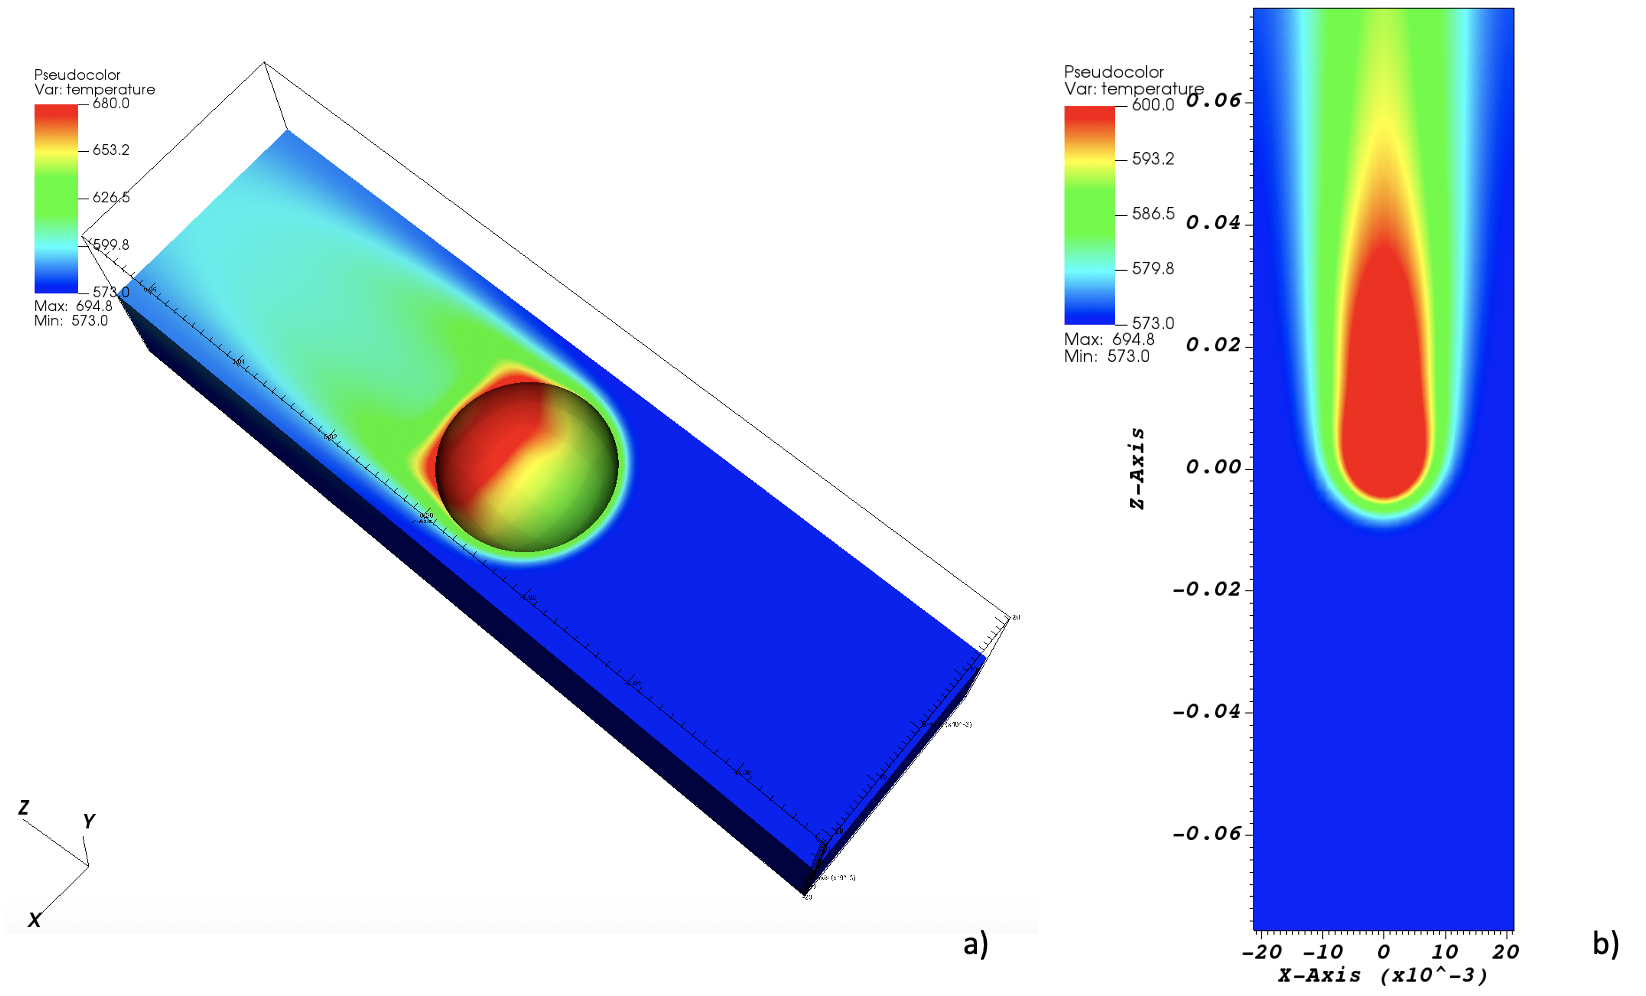
\includegraphics[clip=true,width=0.9\textwidth]{Figures/nrs_vv1}
\caption{Verification test - Single pebble result. a) 3D temperature distribution in the whole domain. b) Cross section at $y=0.016 m$.}
\label{f:nrs1}
\end{figure}

Figure~\ref{f:nrs2} presents a comparison between single pebble results in Cardinal versus results obtained in Nek5000 stand-alone with a conjugate heat transfer mesh. Temperature profiles are compared on a line at $y=0.016 m$ and $x=0 m$ (we note that the domain is centered at the pebble center and the pebble diameter is $D=0.03 m$). We note that the results are nearly identical if a quadratic representation of the surface is employed.

\begin{figure}[!h]
\centering
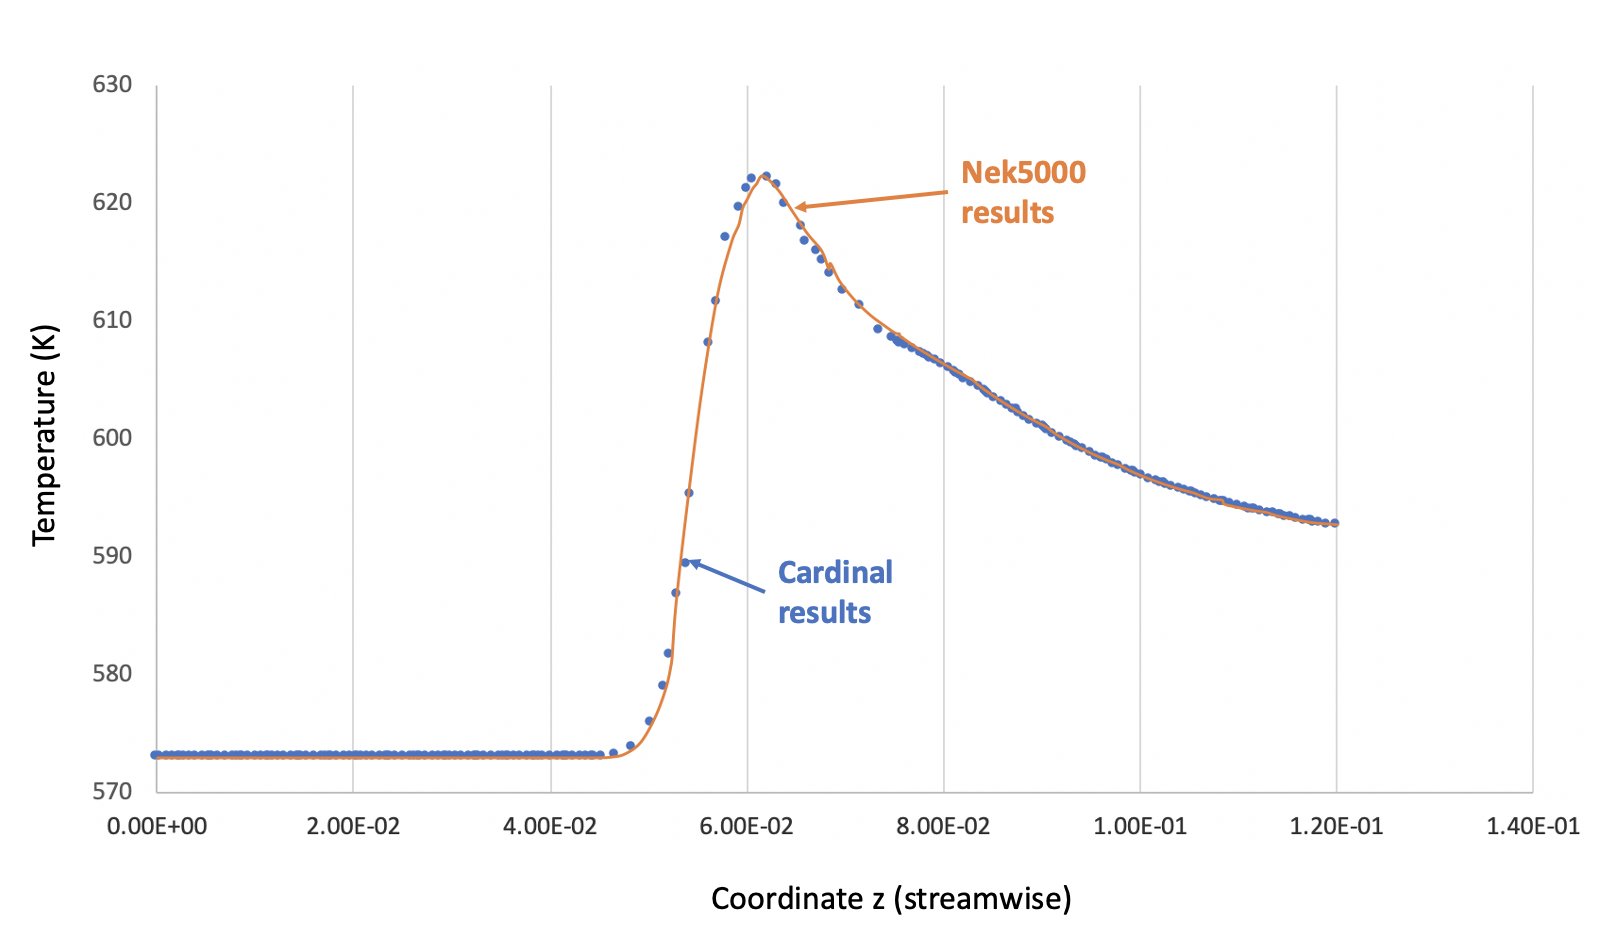
\includegraphics[clip=true,width=0.9\textwidth]{Figures/nrs_vv2}
\caption{Verification test - Single pebble comparison with standalone Nek5000 results. }
\label{f:nrs2}
\end{figure}
